\newpage\subsection*{1551 Worksheet 5 Answers}

\SolutionsStatement

\begin{enumerate}
    
    \item See midterm 1 solutions. 
	\item \begin{enumerate}
    \item \begin{align*} 
    	f'(x) &= \lim_{h\to 0}\frac{f(x+h)-f(x)}{h} \\
        &= \lim_{h\to 0} \frac 1 h \left( \sqrt{5 - x - h} - \sqrt{5-x} \right) \\
        &= \lim_{h\to 0} \frac 1 h \left( \sqrt{5 - x - h} - \sqrt{5-x} \right)\left( \frac{\sqrt{5 - x - h} + \sqrt{5-x}}{ \sqrt{5 - x - h} + \sqrt{5-x} } \right) \\
        &= \lim_{h\to 0} \frac 1 h \left( \frac{(5 - x - h) - (5-x)}{ \sqrt{5 - x - h} + \sqrt{5-x} } \right) \\
        &= \lim_{h\to 0} \left( \frac{-1}{ \sqrt{5 - x - h} + \sqrt{5-x} } \right) \\
        &=  \frac{-1}{ 2\sqrt{5-x} }
    \end{align*}
    
    \item $(-\infty,5]$    
\end{enumerate}
	\item We want points on the curve where $g'(x)$ is equal to the slope of the line $8x - 2y = 1 $.
    \begin{align*}
    	8x - 2y &= 1 \\
        2y &= 8x - 1 \\
        y &= 4x - 1/4
    \end{align*}
    So the slope of the line is 4. 
    \begin{align*}
    	4 &= g'(x) \\
        4 &= \ddx \left(\frac{1}{3}x^3-\frac{3}{2}x^2+1 \right)\\
        4 &= x^2 -3x + 0 \\ 
        0 &= x^2 -3x -4 \\
        0 &= (x+1)(x-4)
    \end{align*}    
    At $x=-1$ and $x=4$ the tangent line has the desired slope. Evaluating $g(x)$ at these points yields the points $(-1,-5/6)$, and $(4,-5/3)$. 
    \newpage 
    
    \item There are many acceptable solutions. But note that for the function to be odd and continuous, it must pass through the origin. 
    
    	\begin{center}
		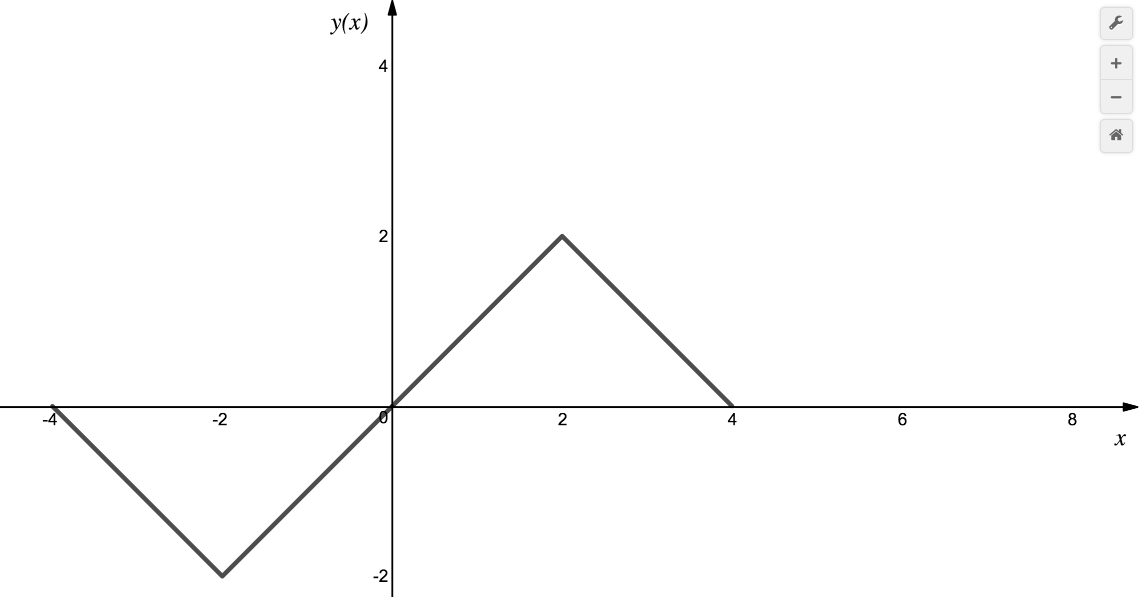
\includegraphics[width=0.85\textwidth]{images/imgWS5OddSpring17.png} 
	\end{center}
    
    \item Many acceptable solutions, including $y(x) = |x-1|$.
    \item \begin{align*}
    f'(x) 
    &= \ddx \ \frac{5x + 1}{4x^2 + 1} \\
    &= \frac{\ddx (5x+1) (5x^2 + 1) - (5x+1)\ddx(4x^2+1)}{(4x^2+1)^2} \\
    &= \frac{5 (5x^2 + 1) - (5x+1)(8x)}{(4x^2+1)^2} \\
    f'(1) &= \frac{5\cdot 6 - 6\cdot 8}{5^2} \\
    &= \frac{30 - 48}{25} \\
    &= -\frac{18}{25}
   \end{align*}
\end{enumerate}




